\chapter{Cara Program}
Tujuan dari buku ini adalah mengajarkan kepada kamu bagaimana berfikir seperti seorang ilmuan komputer. Saya sangat suka bagaimana seorang ilmuan komputer berfikir karena mereka menggabungkan aspek-aspek terbaik dari ilmu Matematika, ilmu Teknik, dan ilmu pengetahuan alam. Sebagaimana halnya Matematikawan, ilmuan komputer menggunakan bahasa formal untuk menyatakan ide khususnya yang berkenaan dengan komputasi. Seperti Insinyur(\textit{Engineer}), ilmuan komputer juga merancang sesuatu, merangkai beberapa komponen kedalam sebuah sistem dan mengeveluasi kelebihan dan kekurangan dari berbagai alternatif solusi. Mirip dengan ilmuan pada umumnya, para ilmuan komputer melakukan observasi tingkah laku dari sistem yang kompleks, membentuk beberap hipotesis dan menguji prediksi yang mereka buat.

Satu-satunya keahlian yang paling penting bagi seorang ilmuan komputer adalah keahlian dalam memecahkan masalah (\textit{problem-solving}). Yang saya maksudkan dengan kemampuan memecahkan masalah adalah kemampuan mereka dalam melakukan formulasi masalah, berfikir secara kreatif mengenai solusi dari masalah yang telah diformulasikan dan mengekspresikan sebuah solusi secara jelas dan akurat.  Dan ternyata proses yang kamu lalui ketika belajar program komputer  adalah sebuah kesempatan yang istimewa  dalam berlatih keahlian memecahkan masalah. Itu kenapa judul dari bab ini adalah "Cara Program".

Pada satu sisi kamu akan belajar pemrograman, yang mana merupkah keahlian yang sangat penting. Disisi lainya, kamu akan menggunakan pemrograman sebagai sarana untuk belajar 

\section{Apa itu bahasa pemrograman?}

Bahasa pemrograman yang akan kamu \textbf pelajari adalah Java, yang termasuk sebuah bahasa pemrograman yang relatif baru (Dirilis pertama kali oleh Sun Microsystem pada may 1995). Java adalah salah satu contoh dari bahasa pemrograman level tinggi (\textit{high-level language}); bahasa pemrograman lain yang juga termasuk kategori bahasa pemrograman level tinggi adalah bahasa Python, C atau C++ dan Perl.

Selain istilah bahasa pemrograman level tinggi, terdapat juga istilah bahasa pemrograman level rendah (\textit{low level languages}) dan terkadang dikenal juga dengan istilah bahasa mesin atau bahasa \textit{assembly}. Pada kenyataanya, komputer hanya bisa memahami bahasa pemrograman level rendah. Oleh sebab itu, sebuah program yang ditulis menggunakan bahasa level tinggi harus diterjemahkan terlebih dahulu ke bentuk bahasa level rendah sebelum program tersebut dijalankan. Proses penterjemahan ini membutuhkan waktu sebelum bisa dijalankan oleh komputer, hal ini menjadi salah satu kekurangan dari bahasa pemrograman level tinggi.

Keunggulan dari bahasa  level-tinggi cukup banyak jika dibandingkan dengan kekuranganna. Pertama, jauh lebih mudah untuk membuat program dengan menggunakan bahasa level-tinggi; waktu yang dibutuhkan untuk menuliskan program jauh lebih singkat, penulisannya juga jauh lebih pendek dan mudah dibaca jika dibandingkan dengan bahasa level-rendah. Keuntungan yang kedua adalah portabilitas dalam menjalankannya diberbagai macam arsitektur komputer dengan tanpa modifikasi. Berbeda halnya dengan program yang ditulis dengan bahasa level-rendah yang hanya bisa dijalankan di komputer tertentu, sehingga perlu dimodifikasi jika ingin dijalankan pada komputer dengan arsitektur yang berbeda.

Oleh karena kelebiha-kelebihan tersebut, maka hampir semua program ditulis dengan menggunakan bahasa pemrograman level-tinggi. Bahasa level-rendah hanya digunakan untuk membuat program-program tertentu saja yang jumlahnya juga sedikit.

Terdapat dua cara untuk menterjemahkan sebuah program; \textbf{interpretasi} (\textit{interpreting}) dan \textbf{kompilasi} (\textit{compiling}). Sebuah \textit{interpreter} adalah sebuah program yang membaca sebuah program level-tinggi dan melakukan apa yang diminta oleh program tersebut. Sebagai akibatnya, interpreter akan menterjemahkan program baris demi baris
Sementara \textit{compiler} adalah sebuah program yang membaca sebuah program level-tinggi dan menterjemahkan keseluruhan program secara langsung, sebelum menjalankan perintah apa pun dari program tersebut. Sering kali, kamu akan melakukan proses kompilasi(\textit{compiling}) secara terpisah terlebih dahulu, kemudian baru  menjalankan (\textit{run}) program. Pada kasus ini, program level-tinggi disebut dengan istilah kode sumber (\textit{source code}) dan program yang telah diterjemahkan disebut dengan istilah kode objek (\textit{object code}) atau \textit{executable}.

Java adalah sebuah bahasa pemrograman yang menggunakan kompilasi dan juga interpretasi ketika menjalankan program. Alih-alih menterjemahkan program ke dalam bahasa mesin, \textit{Java compiler} mengubahnya ke dalam bentuk kode bita (\textit{byte code}). Sama halnya dengan bahasa mesin, kode bita sangat mudah dan juga cepat untuk diterjemahkan (interpretasi). Perbedaannya, kode bita tidak bergantung pada arsitektur komputer tertentu ( lebih \textit{portable}) seperti halnya bahasa level-tinggi. Artinya sebuah kode bita yang dihasilkan di sebuah komputer dapat dipindahkan dan dijalankan di komputer lain yang berbeda mesin/arsitektur. Kemampuan ini merupakan salah satu kelebihan dari bahasa Java jika dibandingkan dengan bahasa level-tinggi lainnya.

\begin{figure}[H]
	\centering 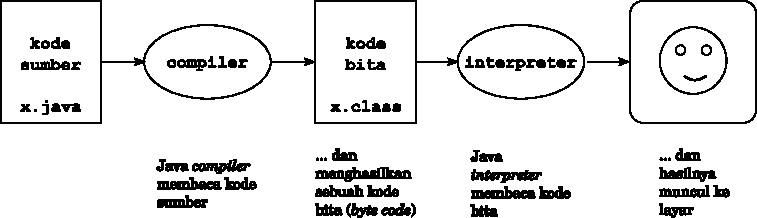
\includegraphics{images/compilingProcess.pdf}
	\caption{Proses kompilasi dan interpretasi pada bahasa Java}
	\label{fig:binaryTreeRekursif}
\end{figure}

Walaupun proses ini terlihat kompleks, namun di beberapa perangkat lunak (\textit{software}) yang digunakan untuk meprograman (sering disebut Integrated Development Environment/IDE) proses-proses tersebut telah dibuat otomatis untuk kamu. Sehingga kamu hanya cukup menekan sebuah tombol "run" saja, maka \textit{software} IDE tersebut akan melakukan kompilasi dan interpretasi untuk program yang kamu buat.Namun disisi lain, kamu tetap harus tahu langkah-langkah yang terjadi dibalik proses yang telah terotomatis tadi, agar ketika terjadi kesalahan maka kamu dapat dengan mudah mengetahui penyebabnya.

\section{Apa itu program?} 

Program adalah sebuah runtutan instruksi yang menyatakan bagaiman melakukan sebuah komputasi \footnote{Definisi ini tidak berlaku untuk seluruh bahasa pemrograman. Sebagai alternatif, lihat $http://en.wikipedia.org/wiki/Declarative\_programming$.}. Istilah komputasi bisa berarti sebagai sesuati yang matematis, seperti menyelesaikan sebuah sistem persamaan atau menemukan akar dari sebuah polinomial, tetapi bisa juga diartikan sebagai sebuah komputasi simbolik, seperti mencari dan mengganti teks pada sebuah dokumen atau mengkompilasi sebuah program. 

Instruksi atau yang sering disebut dengan statemen (\textit{statement}), memilik bentuk yang berbeda-beda untuk setiap bahasa pemrograman, namun terdapat beberapa instruksi dasar yang bisa dilakukan oleh seluruh bahasa pemrograman. instruksi-instruksi dasar tersebut antara lain:

\begin{enumerate}
	\item \textbf{masukan(\textit{input}):} instruksi-instruksi yang digunakan untuk mendapatkan data dari \textit{keyboard} atau sebuah berkas atau dari perangkat lain
	\item \textbf{keluaran (\textit{output}):} instruksi-instruksi yang digunakan untuk menampilkan data kelayar atau mengirimkannya ke berkas atau perangkat lainnya
	\item \textbf{matematika(\textit{math}): }instruksi-instruksi yang digunakan untuk melakukan operasi matematika seperti penjumlahan, pengurangan, perkalian, pembagian dan lainya
	\item \textbf{pengkondisian(\textit{testing}):} instruksi-instruksi yang digunakan untuk memeriksa kondisi tertentu dan menjalankan urutan statemen yang sesuai.
	\item \textbf{perulangan(\textit{repetition}):} instruksi-instruksi yang digunakan untuk melakukan pengulangan terhadap sebuah atau beberapa statemen.
\end{enumerate}

Setiap program yang pernah kamu gunakan, tidak peduli seberapa rumit apapun program tersebut, pasti tersusun dari kombinasi dari instruksi-instruksi dasar di atas. Oleh sebab itu, salah satu cara untuk menjelaskan pemrograman adalah sebagi sebuah proses yang memecah-mecah sebuah pekerjaan yang besar dan kompleks kedalam bentuk beberapa sub pekerjaan yang jauh lebih kecil secara terus menerus hingga sub pekerjaan tersebut dapat secara sederhana dijalankan dengan menggunakan salah satu instruksi-instruksi dasar tadi.

\section{Apa itu \textit{debugging}?}

Untuk alasan lelucon, error (keselahan) yang terdapat pada pemrograman disebut dengan "kutu" (\textit{bug}) dan proses yang dilakukan untuk menemukan dan memperbaik "kutu" tersebut dikenal dengan istilah \textit{debugging}.

Terdapat tiga jenis \textit{error} yang sering muncul dalam sebuah program yaitu \textit{syntax error}, \textit{run-time error} dan \textit{logic dan semantik error}. Penting dan sangat bermanfaat sekali bagi kamu jika kamu bisa membedakan ketiganya,  sehingga kamu dapat dengan cepat dan juga mudah dalam menelusuri kesalahan yang ada dan kemudian memperbaikinya.

\subsection{Kesalahan Sintak \textit{(Syntax Error)}}
\textit{Compiler} hanya bisa melakukan kompilasi jika kode program yang ditulis telah benar secara sintak, jika tidak maka proses kompilasi akan gagal dan kamu tidak akan dapat menjalankan program tersebut. Sintak berarti struktur dan juga aturan dari struktur penulisan dari kode program yang kamu buat.

Sebagai contoh, dalam bahasa inggris sebuah kalimat harus dimulai dengan huruf besar dan diakhiri dengan tanda titik. \\
\texttt{ini adalah contoh kalimat yang salah secara sintak.} \\
\texttt{Ini juga salah secara sintak}

Bagi kebanyakan pembaca, sedikit kesalahan sintak bukanlah masalah yang berarti. Sebagai contoh\textit{ kta msh bsa mmbaca dan memhami tlsan ini dngn baik} walaupu penulisan kata-katanya banyak yang tidak lengkap.

Kemampuan seperti itu tidak dimiliki oleh \textit{compiler}, jika terjadi satu satu kesalahan penulisan (sintak) di kode program yang kamu buat maka \textit{compiler} akan menampilkan pesan error \textit{error message} dan seketika itu akan menghentikan proses kompilasi. Ketika hal tersebut terjadi, maka program yang kamu buat bisa dipastikan tidak akan bisa dijalankan.

Lebih buruk lagi, dalam bahasa Java terdapat lebih banyak aturan sintak dibandingkan dengan sintak yang dimiliki oleh bahasa inggris atau bahasa lainnya, dan pesan error yang tampilkan sering sekali tidak terlalu membantu. Seiring bertambahnya pengalaman kamu, maka kamu akan membuat sedikit kesalahan dan akan lebih cepat dalam menemukannya.
\subsection{Kesalahan ketika menjalankan \textit{(Run-Time Error)}}
Jenis kesalahan berikutnya adalah kesalahan yang muncul ketika menjalankan program (\textit{Run-time Error}). Disebut seperti itu, karena kesalahan tersebut tidak muncul hingga program dijalankan. Di Java, sebuah \textit{run-time error} terjadi ketika \textit{interpreter} menjalankan kode bita (\textit{byte code}) dan terjadi kesalahan dalam proses tersebut.

Java adalah sebuah bahasa pemrograman yang cendrung aman, artinya seluruh potensi kesalahan diupayakan dapat dideteksi oleh \textit{compiler}. Sehingga \textit{run-time error} dapat diminimalisir, khususnya untuk program-program yang sederhana.

Di Java, \textit{run-time error} dikenal ddngan istilah \textit{exceptions}(pengecualian). Dan di banyak lingkungan, \textit{ecxeptions} muncul dalam bentuk \textit{windows} atau \textit{dialog box} yang berisi informasi mengenai apa yang telah terjadi dan apa yang program lakukan ketika hal tersebut terjadi. Informasi ini sangat berguna sekali ketika melakukan \textit{debugging}
\subsection{Kesalahan logika dan semantik \textit{(Logic errors and sematics)}} 
Jenis \textit{error} yang ketiga adalah kesalahan logika dan semantik. Jika program kamu memiliki kesalahan logika, maka program kamu akan dikompilasi dan dijalankan tanpa adanya \textit{error message}, namun tidak akan melakukan apa yang seharusnya. Melainkan akan melakukan hal yang lain. Lebih spesifiknya, program yang kamu buat tidak akan melakukan apa yang kamu perintahkan.

Masalahnya adalah program yang kamu tulis bukanlah program yang kamu inginkan. Hal ini terjadi karena semantik atau makna dari kode program yang kamu buat salah. Menemukan kesalahan logika pada sebuah program adalah hal yang cukup rumit karena kamu harus bekerja secara terbalik, dimulai dari mengidentifikasi keluaran dari program dan mencoba untuk menganalisa apa yang sebenarnya terjadi.

\subsection{Debugging}
Salah satu keahlian yang sangat penting kamu kuasai pada pelajaran ini adalah \textit{debugging}. Walaupun \textit{debugging} bisa jadi membuat kamu frustasi, namun ia merupakan hal yang sangat menarik dan menantang dan merupakan bagian yang sangat bernilai dalam pemrograman.

\textit{Debugging} mirip dengan pekerjaan detektif. Kamu berhadapan dengan petunjuk-petunjuk dan kamu harus menyimpulkan proses serta kejadian yang mengakibatkan hasil yang kamu lihat.

\textit{Debugging} juga serupa dengan ilmu eksperimental (\textit{experimental science}). Disaat kamu mendapati program yang kamu buat mengalami \textit{error}, maka kamu akan membuat semacam dugaan (hipotesis) yang menjadi penyebab dari \textit{error} tersebut, kemudian kamu memodifikasi kode program tersebut berdasarkan hipotesis yang kamu buat, dan kemudian kamu mencoba menjalankan ulang program kamu untuk membuktikan apakah hipotesis kamu benar/tidak. Jika hipotesis kamu benar, maka kamu dapat memprediksi hasil dari modifikasi kamu, dan kamu semakin dekat dengan program yang berfungsi dengan baik. Sebaliknya, jika hipotesis kamu salah, maka kamu harus membuat hipotesis baru untuk kemudian mengulangi proses sebelumnya. Hal ini akan berlangsung secara terus menerus hingga \textit{error} dari program kamu berhasil teratasi. Sebagaimana yang dikatakan oleh \textit{Sherlock Holmes}, "Ketika kamu telah mengeliminasi hal-hal yang tidak mungkin, apa pun yang tersisa walaupun mustahil, haruslah sebuah kebenaran" (dari A. Conan Doyle's \textit{The sign of Four.})

Bagi sebagian orang, pemrograman dan \textit{debugging} adalah hal yang sama. Karena pemrograman adalah sebuah proses \textit{debugging} yang bertahap dari sebuah program hingga program terebut menjalankan apa yang kamu inginkan. Idenya adalah bahwa kamu harus memualai dengan sebuah program yang bisa dijalankan untuk melakukan sesuatu, tidak peduli sekecil apapun yang bisa dilakukan. Kemudian tambahkan modifikasi kecil ke program tersebut diikuti dengan \textit{debugging}, sehingga dengan begitu kamu akan selalu memiliki sebuah program yang berjalan dengan baik dan program yang kamu buat makin lama akan semakin kompleks.

Sebagai contoh, Linux adalah sebuah sistem operasi yang terdiri dari ribuan baris kode program yang pada awalnya hanyalah sebuah program sederhana yang digunakan olen Linus Trovalds untuk mengeksplorasi \textit{chip} Intel 80396. Menurut Larry Greenfield, " Salah satu proyek pertama yang dikerjakan ole Linus adalah sebuah program yang mencetak secara bergantian tulisan AAAA dan BBBB. Kemudian program ini berevolusi menjadi Linux" (dari \textit{The Linux Users' Guide} Beta Version 1).

Pada bab berikutnya, saya menambahkan lebih banyak saran mengenai \textit{debugging} dan praktik-prakatik pemrograman lainnya.


\section{Bahasa Formal dan Bahasa alami}

Bahasa alami adalah bahasa-bahasa yang digunakan oleh orang-orang untuk berbicara, contohnya seperti bahasa Inggris,Spanyol dan Prancis. Bahasa tersebut tidak dirancang oleh manusia, namun berevolusi secara alami.

Bahasa formal adalah bahasa yang dirancang oleh manusia untuk aplikasi-aplikasi yang spesifik. Sebagai contoh,para matematikawan menggunakan bahasa formal dalam bentuk notasi-notasi tertentu untuk menyatakan hubungan antara bebara angka dan simbol. Pra kimiawan menggunakan bahasa formal untuk mereprsentasikan struktur kimiawi dari molekul-molekul. Dan yang paling penting adalah, 

\textbf{Bahasa pemrograman adalah bahasa formal yang telah dirancang untuk mengekspresikan komputasi}

Bahasa formal memiliki aturan sintak yang ketat. Sebagai contoh, $3+3=6$ adalah pernyataan matematika yang benar secara sintak, sedangkan $ 3\$=$ merupakan pernyataan yang salah. Begitu halnya juga dengan $H_{2}O$ adalah sebuah pernyataan nama zat kimia yang benar, namun tidak halnya untuk $_{2}Z_{z}$.

Aturan sintak terdiri dari dua hal yaitu aturan yang berkaitan dengan simbol(\textit{token}) dan yang berkaitan dengan struktur. Toke merupakan elemen dasar dari sebuah bahasa, seperti halnya kata, angka, dan elemen kimiawi. Masalah yang terdapat pada pernyataan matematika $ 3\$=$ adalah $ \$ $ merupakan bukan token yang legal dalam matematika (paling tidak sejauh yang saya tahu). Begitu halnya dengan $_{2}Z_{z}$, tidak legal karena tidak ada elemen kimia yang memiliki singkatan $ Z_{z} $.

Aturan yang kedua adalah aturan yang berkenaan dengan struktur dari sebuah pernyataan, yaitu mengenai bagaimana token-token disusun. Pernyataan matematika $ 3\$=$ adalah pernyataan yang tidak legal secara struktur, karena kamu tidak dapat meletakkan tanda sama dengan (=) di akhir dari sebuah pernyataan matematis. Sama halnya dengan penulisan $_{2}Z_{z}$ adalah tidak legal secara struktur, karena tidak boleh menempatkan \textit{superscript} di posisi paling depan.

Ketika kamu membaca sebuah kalimat di bahasa Inggris atau pernyataak di bahasa formal, kamu harus mencari tahu atau memahami struktur dari kalimat tersebut (walaupun dalam bahasa alami kamu melakukannya secara tidak sadar). Proses seperti ini dikenal dengan istilah \textit{parsing} (penguraian kalimat).

Walaupun bahasa alami dan bahasa formal memiliki kesamaan yang bersifat umum dalam hal token, struktur, sintak dan semantik, namun ada beberapa hal yang menjadi pembedanya, sebagaimana yang dijelaskan berikut;
ambiguity(keambiguan):bahasa alami 


